\documentclass[12pt]{article}

\usepackage[spanish]{babel}
\usepackage[utf8]{inputenc}
\usepackage{graphicx}
\usepackage{geometry}
\usepackage{xcolor}
\usepackage{fancyhdr}
\usepackage{lastpage}
\usepackage{pdfpages}
\usepackage{listings}
\usepackage{schemata}

\geometry{top=25mm,left=15mm,right=15mm,a4paper}

\pagestyle{fancy}
\fancyhf{}
\lhead{Analisis de Algoritmos}
\cfoot{Página \thepage\ de \pageref{LastPage}}

\graphicspath{./}

\begin{document}
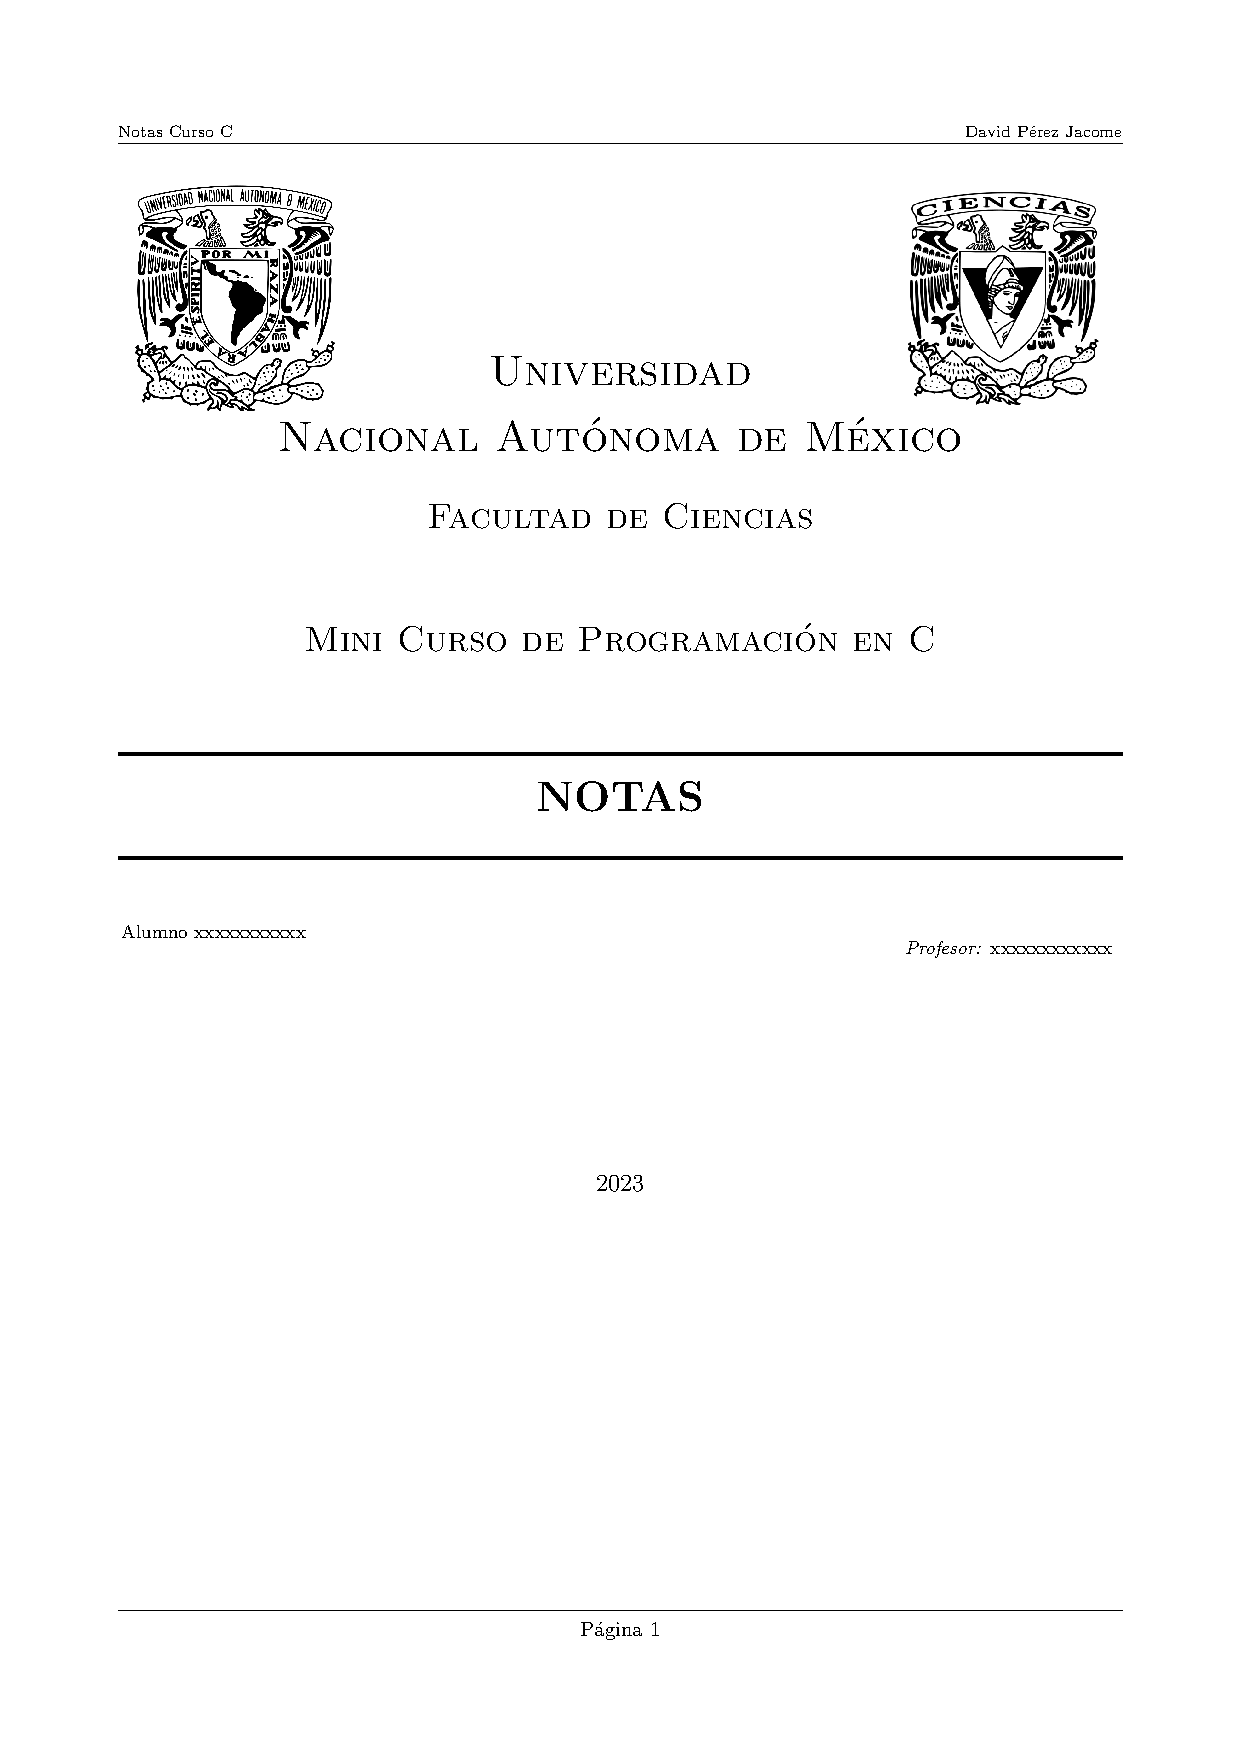
\includepdf{Portada.pdf}
{\color{blue} \section*{\textbf{Notas del Curso de Aprender a Programar con C.}}}
\vspace{1em}

{\color{red} \subsection*{\textbf{INTRODUCCIÓN.}}}

Inicialmente me di a la tarea de escribir este pequeño curso para futuras generaciones que  quieran aprender a programar y no sepan el como empezar, de igual 
manera es un pequeño repaso pasa fundamentar las bases de un buen curso, cabe recalcar que me guie de un curso en ingles de la plataforma \textbf{COURSERA} "Programming Fundamentals".\\

En este curso como lo describe perfectamente el titulo vamos a sembrar los fundamentos generales que nos van a servir para aprender a programar, como estudiante de Ciencias de la Computación tratare de ser lo más descriptivo y claro que me sea 
posible pero si en algún momento no es el caso y esta costando trabajo, me pueden contactar a traves de la dirección de correo electronico: \textbf{david1956@ciencias.unam.mx} y con gusto podre orientarlos en el contenido de este mini curso.\\











\end{document}